\subsection{Inversão das Linhas Pares}

Inverte todas as linhas pares horizontalmente.

\begin{figure}[h]
    \centering
    \begin{subfigure}{0.45\textwidth}
        \centering
        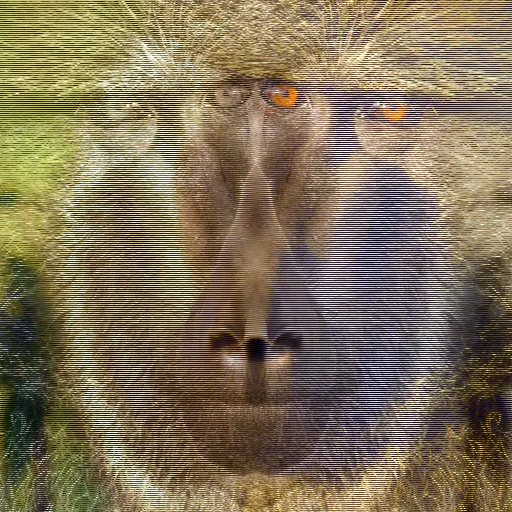
\includegraphics[width=6cm]{resultados/colorinvp.png}
        \caption{\texttt{imagens/color.png}}
    \end{subfigure}%
    \begin{subfigure}{0.45\textwidth}
        \centering
        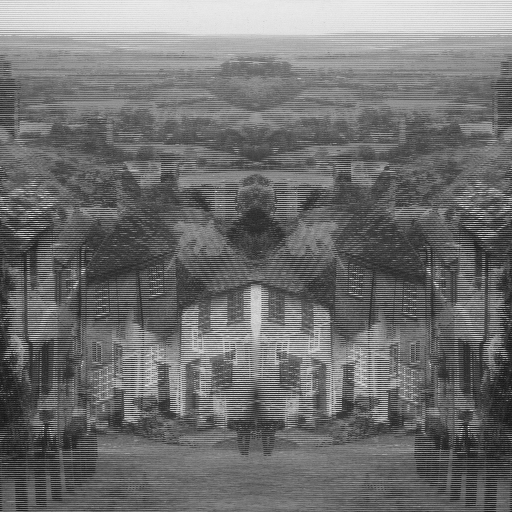
\includegraphics[width=6cm]{resultados/cityinvp.png}
        \caption{\texttt{imagens/city.png}}
    \end{subfigure}

    \caption{Linhas pares invertidas.}
\end{figure}

\begin{listing}[H]

    \begin{minted}{python}
        def inverte_linhas_pares(imagem):
            magem[::2] = image[::2,::-1]
            return imagem
    \end{minted}

    \caption{Comando \texttt{inverte.pares}}
\end{listing}
